\chapter{Model training and device classification results} \label{chap6}

In the previous chapters we described how to create a Neural Network classifier able to solve the device identification task and how to obtain and preprocess a dataset to train the classifier on. In this chapter we present and discuss the results of the training of the classifier models on the two proposed dataset alongside with an evaluation of their performances.

As said before, the results presented in this chapter are obtained after dividing the datasets in three subsets: the training set over which the classifier are trained, the validation set, used to monitor the performances during the training and the test set, used to evaluate the real performances of the classifiers.

In section \secref{res_lb} we discuss the choice of the architecture depending on the lookback value $L$ and how the choice of the latter can impact the training of the selected architecture. In \secref{res_test} we will then recall the main features of the selected architectures and show the results of the classifiers training, alongside with their final performances. Finally in \secref{res_unseen} we will presents the results of the implementation of the trained classifier for the identification of devices not included in the original dataset. All the computations have been performed on a machine with a Ryzen 6 core CPU, an NVIDIA GTX 1660 Super GPU and 32GB of memory.


\section{Classifier architecture and time series length}\label{res_lb}

In \chapref{chap4} we presented the statistic and class division of the 4SICS and IoT Sentinel dataset, respectively in \tabref{tab:4sicsdev} and \tabref{tab:iotdev}. During the preprocessing operation the 4SICS dataset timeseries were created using a value of the lookback, defined in \secref{fig:ts_processing}, of $L=100$. The IoT dataset on the other hand was preprocessed using a value of $L=30$. As previously stated the choice of using a smaller lookback value is made in order to maximize the number of obtained timeseries and, consequently, the dataset dimension, with the goal of maximizing the final performance of the model. 

This choice however is not compatible with the use of the 1B\_AP architecture, namely the general proposed model, so the 1B\_NP architecture should be used instead. The reason for the incompatibility of the 1B\_AP architecture with a value $L=30$ is the presence of the pooling layers. 
Even when using a poolsize of 2, the smallest possible value, each layer halves the size of the vector. This fact, combined with the size reduction caused by the filters\footnote{In the 1B\_AP architecture the zero padding technique is not implemented since we want to reduce the input dimensionality. Indicating with $K$ the size of the filter, after a convolutional layers the size of the input and output vector will the differ by $K-1$.}, results in a too low final dimension of the input or, in some cases, even in the mathematical incompatibility of the operations.

The chosen value of $L=30$ corresponds to the lowest value for which the training performance of the model is not critically affected. This value was estimated training several 1B\_NP classifiers using samples obtained from the dataset preprocessing with different values of $L$. The dataset used for this estimation is the 4SICS dataset, in order to avoid possible biases caused by the training dataset size. 
In \figref{fig:res_lb_val} the loss function and model accuracy, for different lookback values, over the training and validation dataset is shown. As we can see from these plots  using values of $L=10,20$ results in divergence of the training and validation loss function. This behaviour indicates the presence of overfitting during the training. This may be explained considering that, for low $L$ valus some variety is lost in the time series, resulting in a too high model complexity for the provided input dimension.

The classifier trained with $L=30$ on the other hand does not present such behaviour, justifying the choice made for the lookback value for this architecture. Additional plots of the loss function and model accuracy for higher values of the lookback are shown in \appref{app:lb_bonus_res}.


\begin{figure}[!h]
    \centering
    \begin{minipage}[c]{0.49\textwidth}
        \vspace{0pt}
        \centering
        \subfloat[Loss function with lookback $L=10$]{
        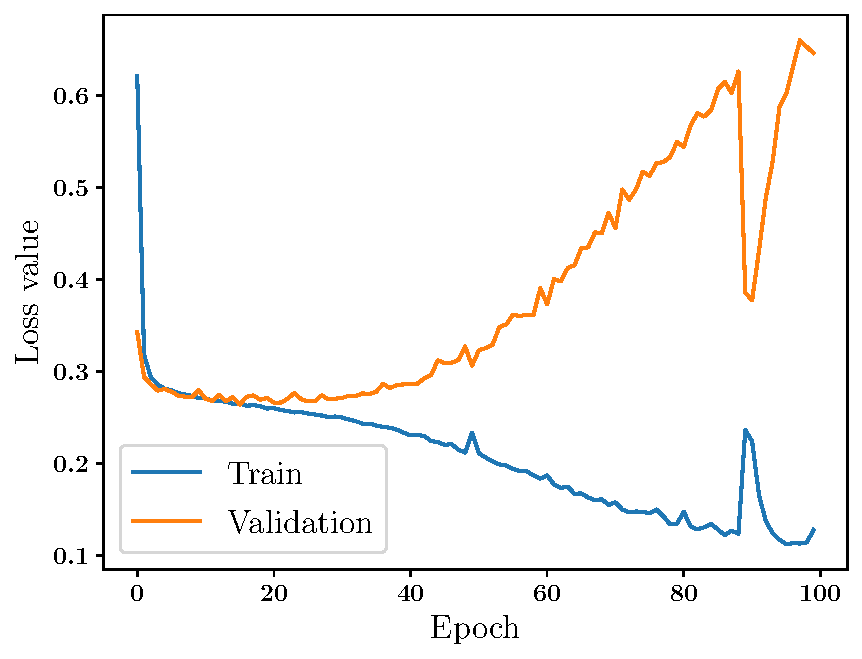
\includegraphics[width=\textwidth]{images/results/LB_test_10_20210613-180735__type_1branch_no_pool__st_scale_sub__lb_10__act_elu__nf_16__ks_10__nn_50__l2_1e-05__bs_200__ep_100__loss.pdf}
            \label{fig:lb_10_loss}
        }
    \end{minipage}%
    \hfill%
    \begin{minipage}[c]{0.49\textwidth}
        \vspace{0pt}
        \centering
        \subfloat[Accuracy with lookback $L=10$]{
        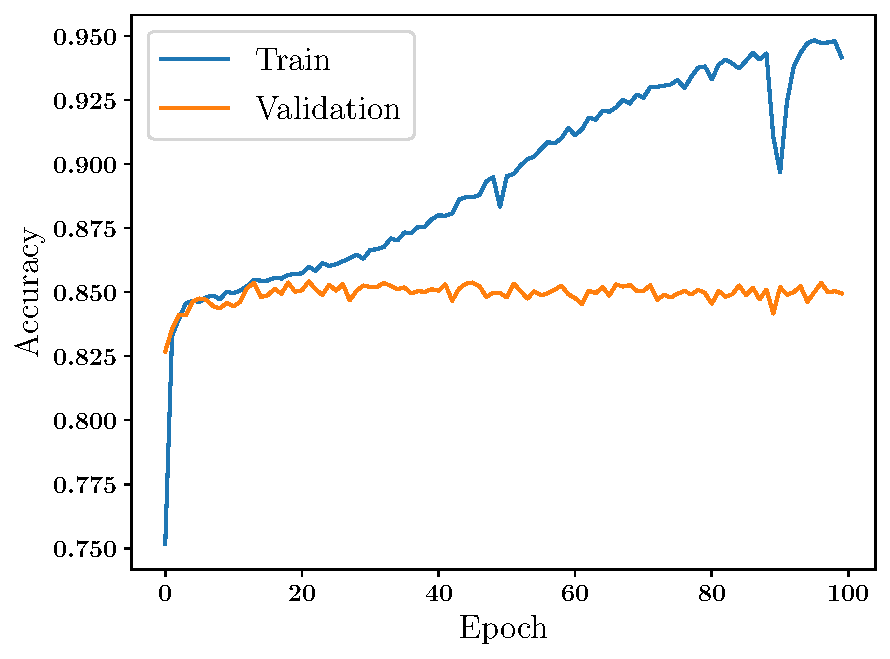
\includegraphics[width=\textwidth]{images/results/LB_test_10_20210613-180735__type_1branch_no_pool__st_scale_sub__lb_10__act_elu__nf_16__ks_10__nn_50__l2_1e-05__bs_200__ep_100___accuracy.pdf}
            \label{fig:lb_10_acc}
        }
    \end{minipage}
        \begin{minipage}[c]{0.49\textwidth}
        \vspace{0pt}
        \centering
        \subfloat[Loss function with lookback $L=20$]{
        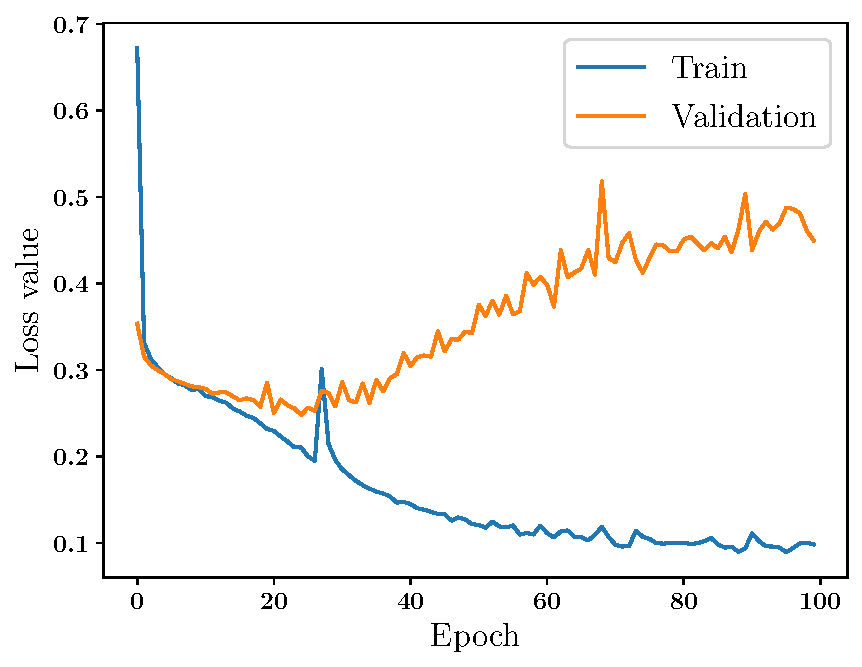
\includegraphics[width=\textwidth]{images/results/LB_test_20_20210613-180946__type_1branch_no_pool__st_scale_sub__lb_20__act_elu__nf_16__ks_10__nn_50__l2_1e-05__bs_200__ep_100__loss.pdf}
            \label{fig:lb_20_loss}
        }
    \end{minipage}%
    \hfill%
    \begin{minipage}[c]{0.49\textwidth}
        \vspace{0pt}
        \centering
        \subfloat[Accuracy with lookback $L=20$]{
        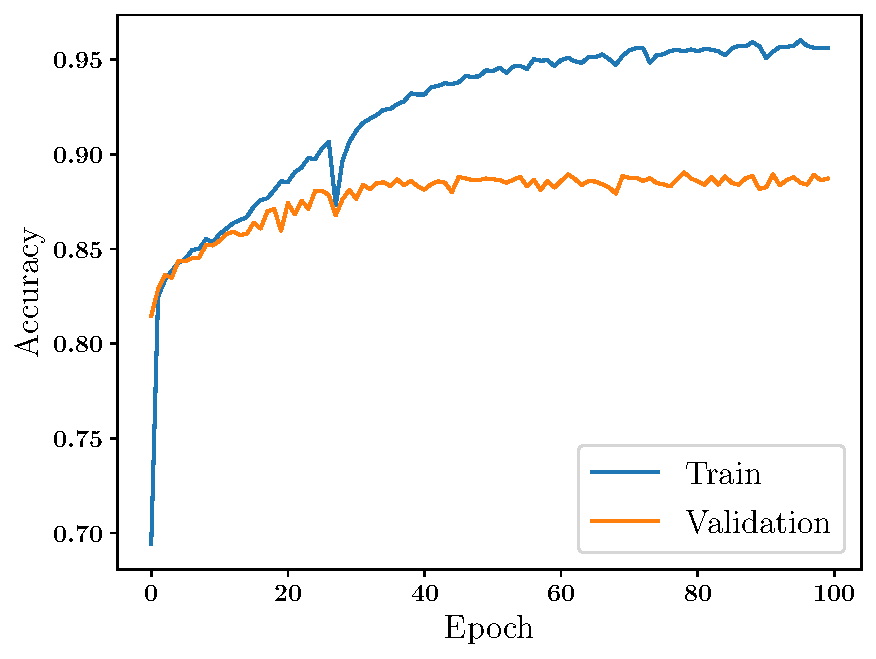
\includegraphics[width=\textwidth]{images/results/LB_test_20_20210613-180946__type_1branch_no_pool__st_scale_sub__lb_20__act_elu__nf_16__ks_10__nn_50__l2_1e-05__bs_200__ep_100___accuracy.pdf}
            \label{fig:lb_20_acc}
        }
    \end{minipage}    \begin{minipage}[c]{0.49\textwidth}
        \vspace{0pt}
        \centering
        \subfloat[Loss function with lookback $L=30$]{
        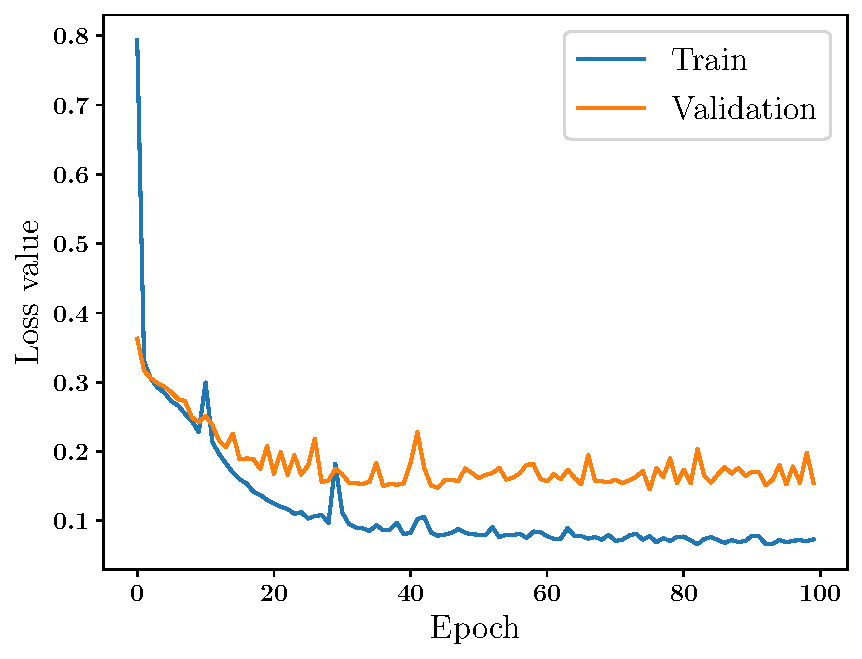
\includegraphics[width=\textwidth]{images/results/LB_test_30_20210613-181249__type_1branch_no_pool__st_scale_sub__lb_30__act_elu__nf_16__ks_10__nn_50__l2_1e-05__bs_200__ep_100__loss.pdf}
            \label{fig:lb_30_loss}
        }
    \end{minipage}%
    \hfill%
    \begin{minipage}[c]{0.49\textwidth}
        \vspace{0pt}
        \centering
        \subfloat[Accuracy with lookback $L=30$]{
        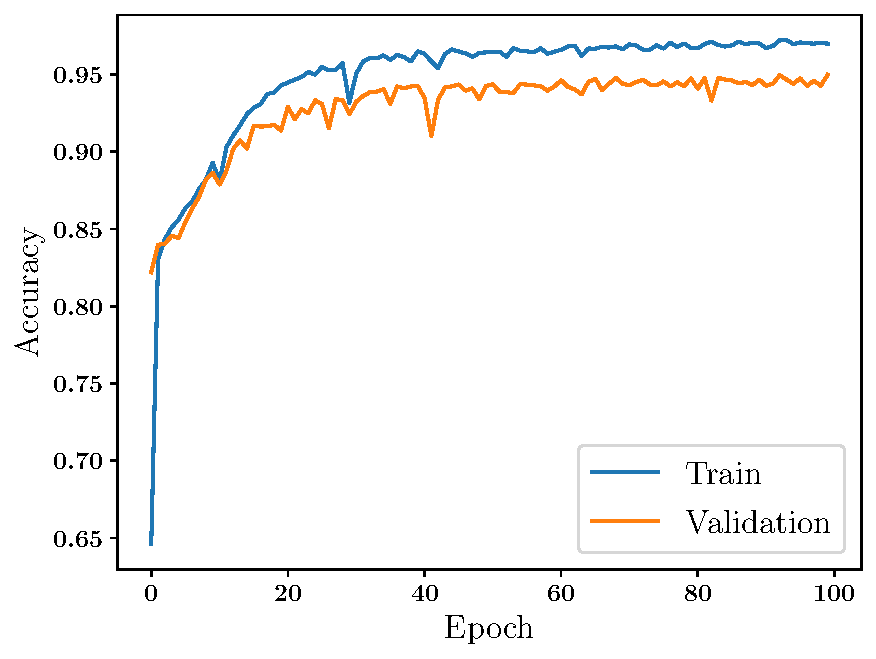
\includegraphics[width=\textwidth]{images/results/LB_test_30_20210613-181249__type_1branch_no_pool__st_scale_sub__lb_30__act_elu__nf_16__ks_10__nn_50__l2_1e-05__bs_200__ep_100___accuracy.pdf}
            \label{fig:lb_30_acc}
        }
    \end{minipage}


    \caption{lookback analysis}
    \label{fig:res_lb_val}
\end{figure}





\section{Model training and final performance}\label{res_test}

In this section we present the final performance of the proposed classifier after the training procedure for both datasets. The performances have been evaluated used the test sets and the possible presence of over or under fitting behaviour is monitored, as shown previously, using the validation set.



\subsection{4SICS dataset}

As stated previously the chosen architecture for the device classification over the 4SICS dataset in the 1B\_AP model, namely an architecture with one convolutional "branch" with average pooling layers. The selected device classes, shown in \tabref{tab:4sicsdev}, have been preprocessed using a lookback $L=100$. The training was performed for 300 epochs using a batch size \footnote{The batch size indicated after how many samples the free parameters of the Neural Networks should be updated using the backpropagation algorithm} of 200. 

In \figref{fig:4sics_results} the evolution of the loss function and of the model accuracy over the training and validation set are shown. As we can see the model is able to reach high performances and does not show overfitting behaviour. 


\begin{figure}[h]
    \centering
    \begin{minipage}[c]{0.49\linewidth}
        \vspace{0pt}
        \centering
        \subfloat[Loss function during training]{
        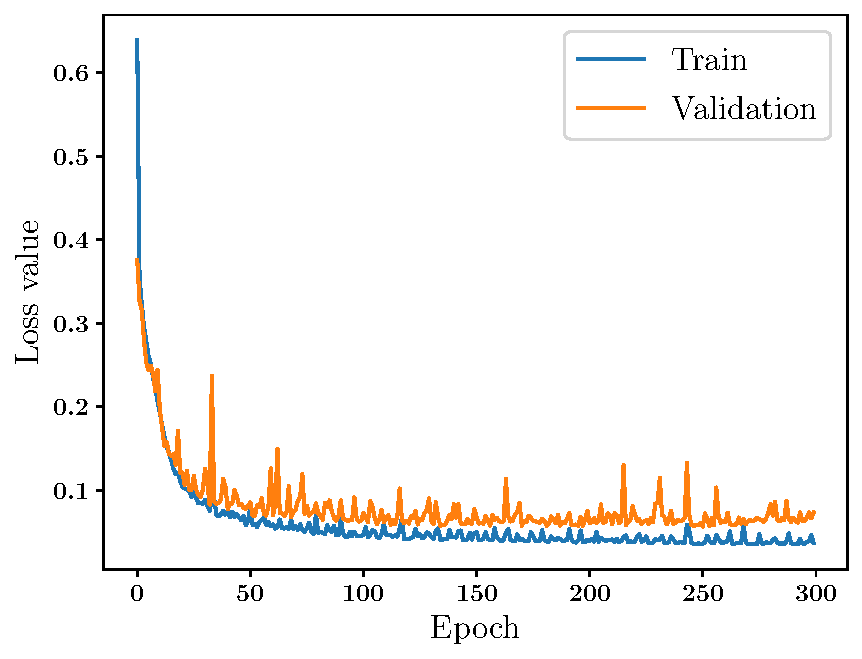
\includegraphics[width=\textwidth]{images/results/4SICS_clasf_20210613-174409__type_1branch__st_scale_sub__lb_100__act_elu__nf_16__ks_10__nn_50__l2_1e-05__bs_200__ep_300__loss.pdf}
            \label{fig:4sics_loss}
        }
    \end{minipage}%
    \hfill%
    \begin{minipage}[c]{0.49\linewidth}
        \vspace{0pt}
        \centering
        \subfloat[Accuracy during training]{  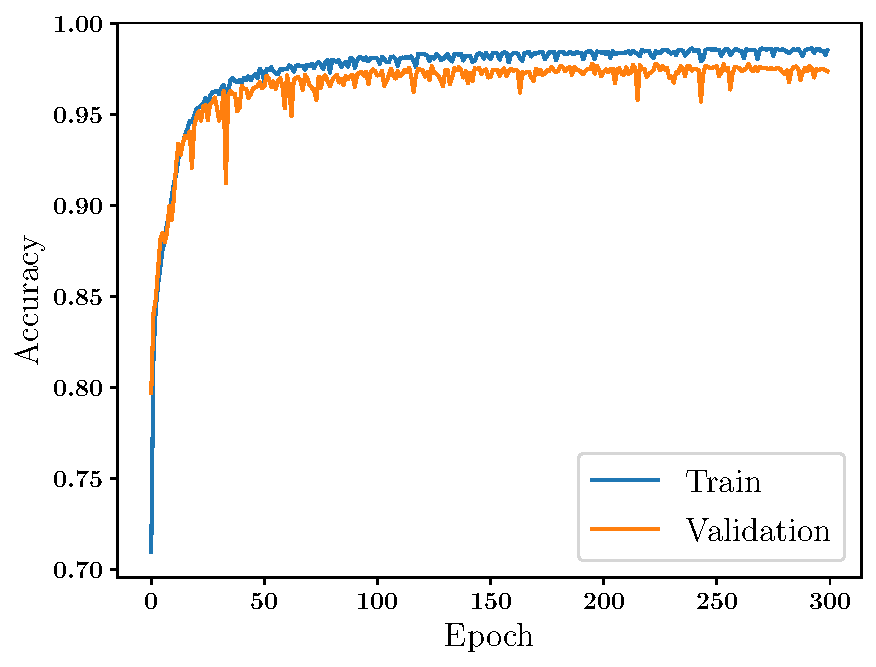
\includegraphics[width=\textwidth]{images/results/4SICS_clasf_20210613-174409__type_1branch__st_scale_sub__lb_100__act_elu__nf_16__ks_10__nn_50__l2_1e-05__bs_200__ep_300___accuracy.pdf}
        \label{fig:4sics_loss}
        }
    \end{minipage}%
    \caption{confronto}
    \label{fig:4sics_results}
\end{figure}

The model performances are evaluated over the test dataset comparing the predicted class of the devices with their true class. This comparison is done using a confusion matrix, shown in \figref{fig:4sics_results_cm}. As we can see for all classes more than 90\% of the predicted labels are correct with the Switch and Router class having 100\% correct predictions. From this matrix we also estimate a 96.2\% overall test accuracy.

\begin{figure}[h]
    \centering
        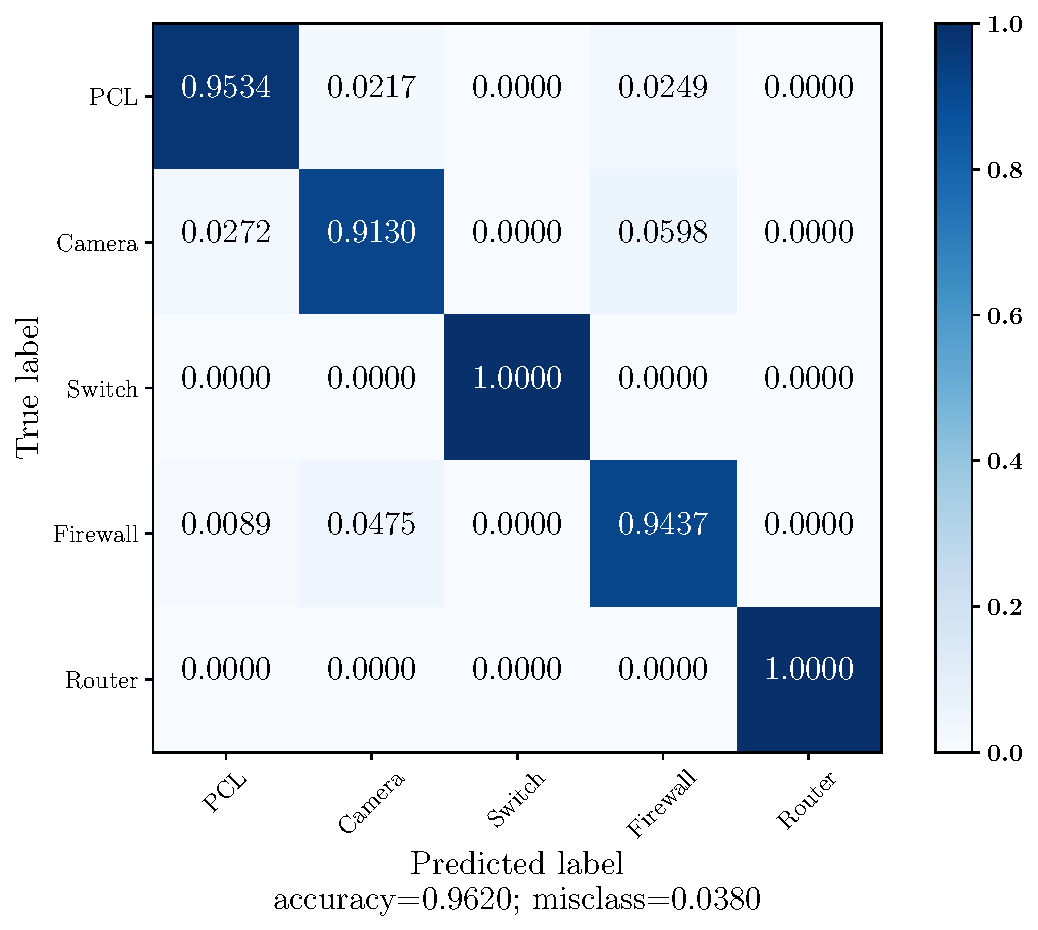
\includegraphics[width=0.6\textwidth]{images/results/4SICS_clasf_20210613-174409__type_1branch__st_scale_sub__lb_100__act_elu__nf_16__ks_10__nn_50__l2_1e-05__bs_200__ep_300___cm.pdf}
    \caption{confronto}
    \label{fig:4sics_results_cm}
\end{figure}

\subsection{IoT dataset}

As stated previously due to the small length of the timeseries the chosen architecture for the device classification over the IoT Sentinel dataset in the 1B\_NP model, namely an architecture with one convolutional "branch" without pooling layers. The selected device classes, shown in \tabref{tab:iotdev}, have been preprocessed using a lookback $L=30$. The training was performed for 300 epochs using a batch size of 100. 

In \figref{fig:iot_results} the evolution of the loss function and of the model accuracy over the training and validation set are shown. As for the previous dataset the model is able to reach high performances and does not show overfitting behaviour, validating the choice of architecture and lookback value. 


\begin{figure}[h]
    \centering
    \begin{minipage}[c]{0.49\linewidth}
        \vspace{0pt}
        \centering
        \subfloat[Loss function during training]{
        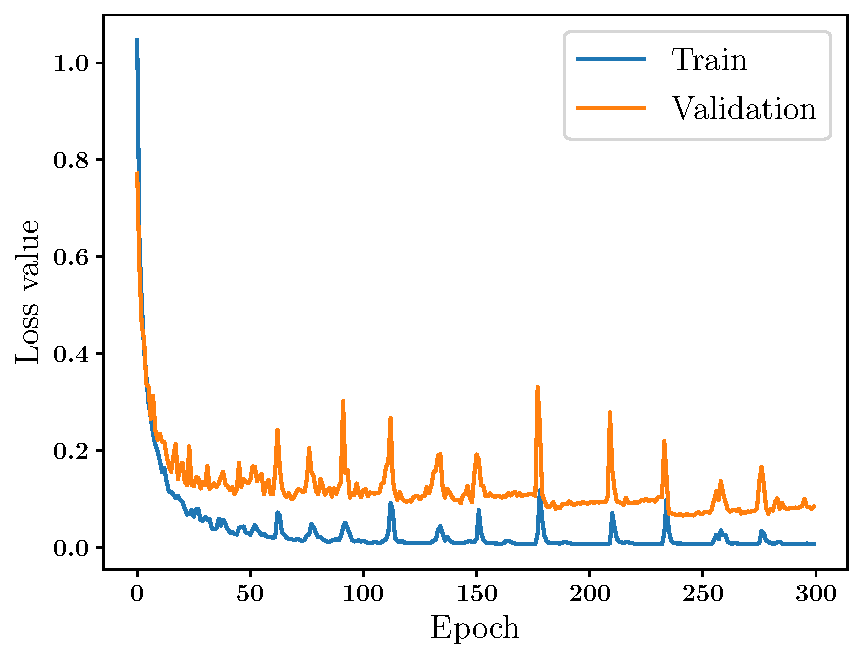
\includegraphics[width=\textwidth]{images/results/IoT_clasf_20210613-175027__type_1branch_no_pool__st_scale_sub__lb_30__act_elu__nf_16__ks_10__nn_50__l2_1e-05__bs_200__ep_300__loss.pdf}
            \label{fig:iot_loss}
        }
    \end{minipage}%
    \hfill%
    \begin{minipage}[c]{0.49\linewidth}
        \vspace{0pt}
        \centering
        \subfloat[Accuracy during training]{  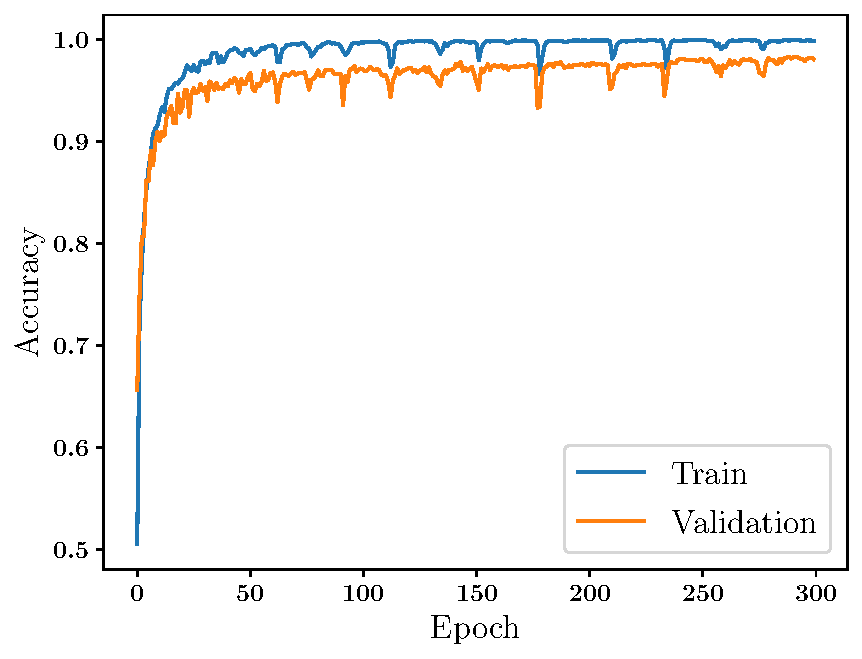
\includegraphics[width=\textwidth]{images/results/IoT_clasf_20210613-175027__type_1branch_no_pool__st_scale_sub__lb_30__act_elu__nf_16__ks_10__nn_50__l2_1e-05__bs_200__ep_300___accuracy.pdf}
        \label{fig:iot_loss}
        }
    \end{minipage}%
    \caption{confronto}
    \label{fig:iot_results}
\end{figure}


As for the previous model we evaluate the model performances using a confusion matrix, shown in \figref{fig:4sics_results_cm}. For this dataset the classifier is able to reach a test accuracy higher than 95\% for all the classes with an overall accurcay of 98.6\%

\begin{figure}[h]
    \centering
        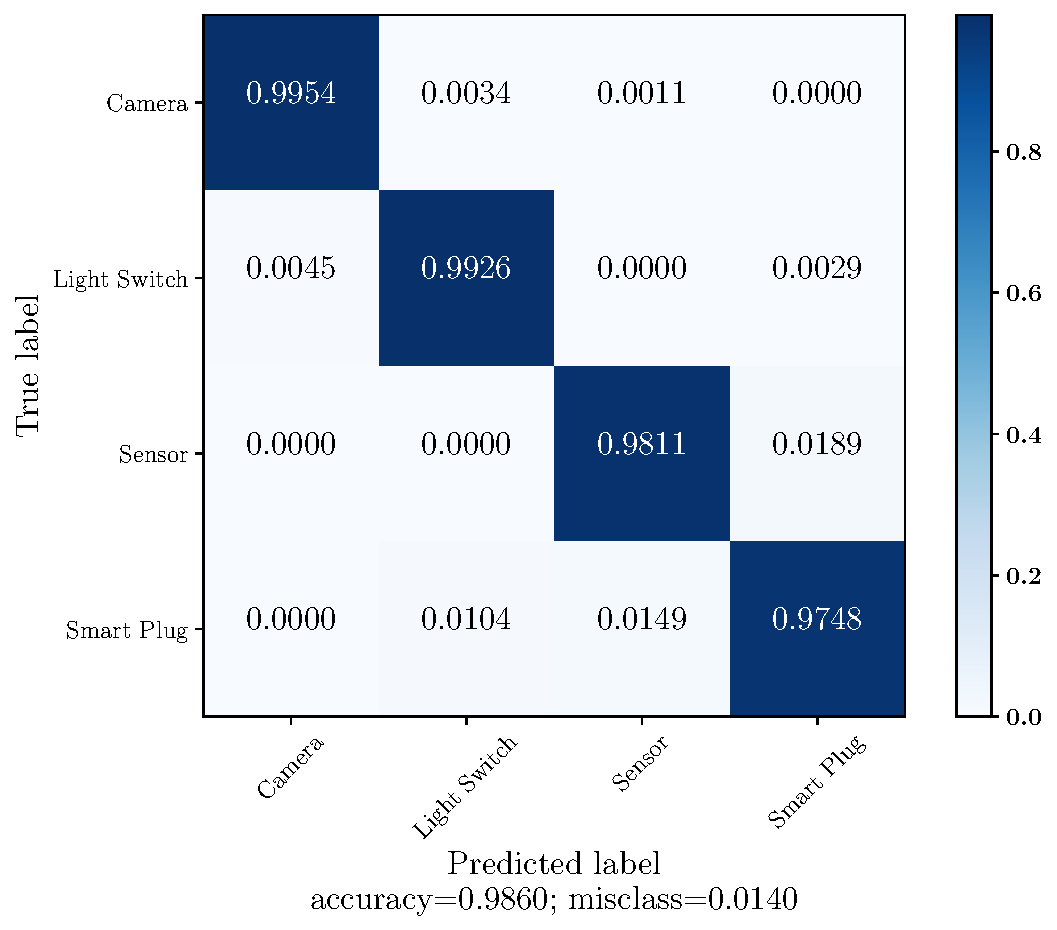
\includegraphics[width=0.6\textwidth]{images/results/IoT_clasf_20210613-175027__type_1branch_no_pool__st_scale_sub__lb_30__act_elu__nf_16__ks_10__nn_50__l2_1e-05__bs_200__ep_300___cm.pdf}
    \caption{confronto}
    \label{fig:iot_results_cm}
\end{figure}



\section{"Unseen" device classification}\label{res_unseen}

In the previous section we show that the proposed model is able, with great accuracy, of correctly of performing the identification of a device. We now want to try to use the trained model in order to classify an "unseen" device.

More precisely we are interested in taking a processing the time series from device that were not included in the previously described datasets but that bolong to one of the classes the classifier was trained to distinguish. Our goal is to see if the classifier is able to recognize similarities between the device he was trained on and completely new devices. This test has a is particularly interesting due to how it translates in a real world application. In the real world in fact we can create more powerful classifiers using deeper architecture but mostly creating very big datasets with tens if not hundreds of devices inside. The OT and IoT worlds however are continuously evolving and new devices are developed each year. The ability of the classifier of identifying a completely new device will then be fundamental in order for the model to keep his performances at the expected level when new devices are introduced in a network. 

For each dataset we chose two different devices that were not part of the datasets described in \tabref{tab:4sicsdataset} and \tabref{tab:iotdataset} and processed their time series using exactly the same procedure. After this we used the trained classifiers to predict the class of each processed time series. The final class prediction will then be the class with the highest number of time series assigned. The result are shown as histogram in \figref{fig:4sics_unseen} and \figref{fig:iot_unseen} respectively for the 4SICS and IoT dataset. 



\begin{figure}[h]
    \centering
    \begin{minipage}[c]{0.49\linewidth}
        \vspace{0pt}
        \centering
        \subfloat[Class prediction of an "unseen" PLC]{
        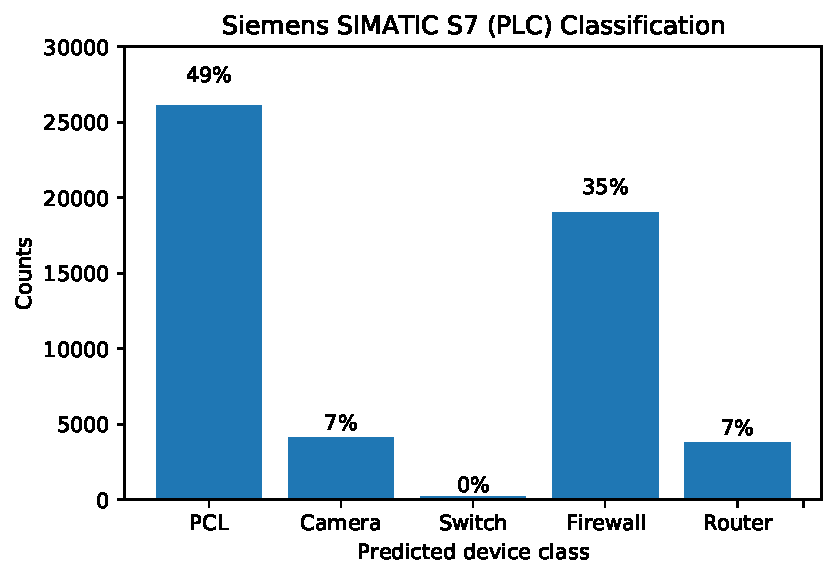
\includegraphics[width=\textwidth]{images/results/4sics_clasf_plc1_recognition.pdf}
            \label{fig:4sics_unseen_plc}
        }
    \end{minipage}%
    \hfill%
    \begin{minipage}[c]{0.49\linewidth}
        \vspace{0pt}
        \centering
        \subfloat[Class prediction of an "unseen" Router]
        {  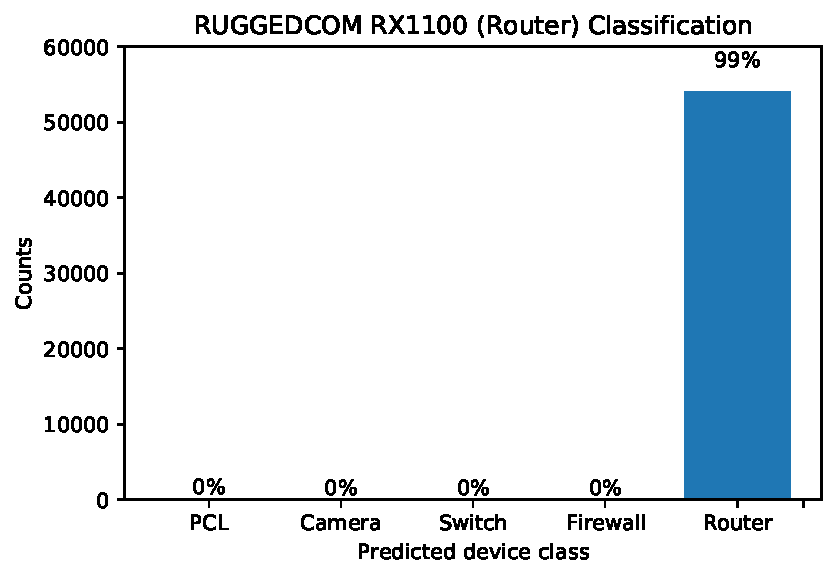
\includegraphics[width=\textwidth]{images/results/4sics_clasf_router_recognition.pdf}
            \label{fig:4sics_unseen_router}
        }
    \end{minipage}%
    \caption{confronto}
            \label{fig:4sics_unseen}
\end{figure}


\begin{figure}[h]
    \centering
    \begin{minipage}[c]{0.49\linewidth}
        \vspace{0pt}
        \centering
        \subfloat[Class prediction of an "unseen" Camera]{
        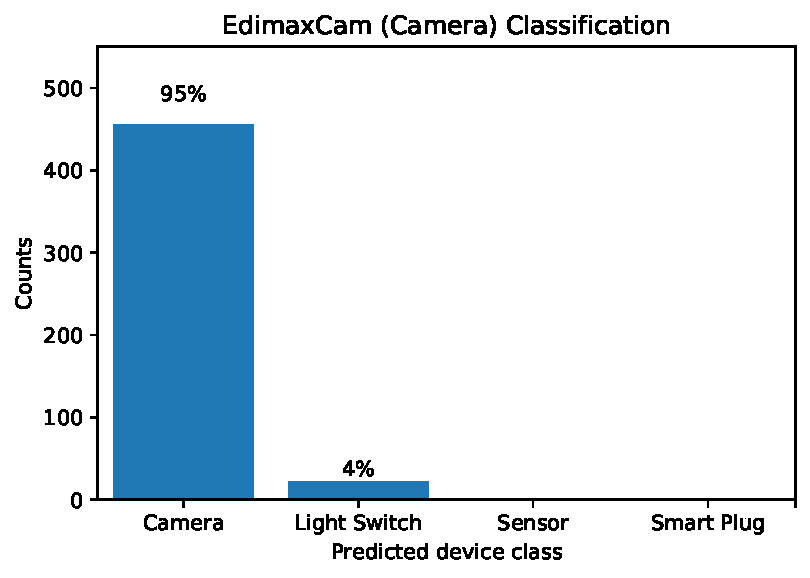
\includegraphics[width=\textwidth]{images/results/iot_clasf_cam_recognition.pdf}
            \label{fig:iot_unseen_camera}
        }
    \end{minipage}%
    \hfill%
    \begin{minipage}[c]{0.49\linewidth}
        \vspace{0pt}
        \centering
        \subfloat[Class prediction of an "unseen" Light Switch]
        {  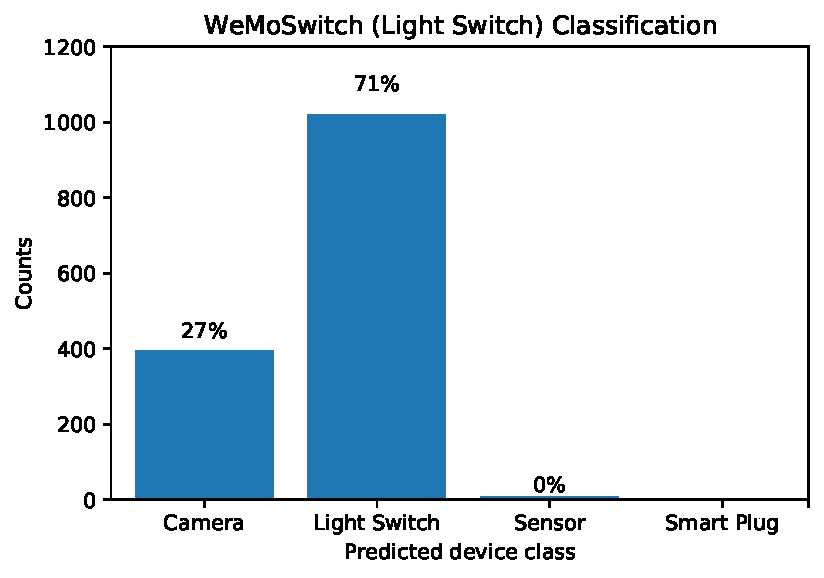
\includegraphics[width=\textwidth]{images/results/iot_clasf_switch_recognition.pdf}
            \label{fig:iot_unseen_light}
        }
    \end{minipage}%
    \caption{confronto}
            \label{fig:iot_unseen}
\end{figure}

As we can see in all four cases the trained classifiers are able to correctly classify the device. It is however important to notice that not all the predictions are done with the same accuracy. More specifically we can see that for the devices belonging to the Router and Camera class more than 95\% time series have been correctly classified. The devices belonging to the PLC and Light Switch class on the other hand despite being correctly classified present a non negligible fraction of missclassified time series.

This can be expected since we are considering devices that were not part of the training dataset and the ability alone of the classifier of correctly identifying them is already a great achievement. More precise classification can probably using larger training dataset with more considered devices in different network configurations.


\section{Discussion}

In the previous sections we evaluated the performances of the proposed architectures over the two datasets. The results show that the classifiers are able to solve the identification task with grate test accuracy. Looking at the loss function and accuracy plot we see a regular behaviour allowing us to exclude the presence of over or under fitting behaviuor. This fact, alongside with the overall test accuracy obtained, validates the choice made for the architecture and lookback value in both situations.

Looking at the presented confusion matrices we estimated the overall test accuracy obtaining very high accuracy values in both cases. This translates, in a real world application, in the ability, of a trained classifier, in correctly recognizing a device that was included in its training dataset with great precision.

The use of trained classifier to identify devices that were not included in the training dataset show that the proposed architectures are able to recognize similarities in the device behaviour and, consequently, of correctly classifying them. This result is really important since demonstrates the capability of a trained classifier to easily adapt to new devices that can be introduced inside of a network and that may not have been included in its training dataset. In a real world application this translate in the possibility of truly implementing this type of classifier and a device identifier without the necessity of executing a new training procedure whenever a new device is connected to the network.